
\chapter{基于后缀树的重复记录检测}
\label{chap:suffixtree}

\section{后缀树简介}
\label{sec:suffixtreeintro}
后缀树(Suffix Tree)是一种可以快速高效实现许多字符串操作的数据结构。Weiner最早
在\cite{weiner1973linear}中提出了后缀树的概念,Ukkonen在\cite{ukkonen1995line}中
提出了一个$O(n)$时间复杂度的在线构造算法。

后缀树实际上是前缀树(Trie树)的一种特殊形式。后缀树的每一条边都代表着一个序列,从
根节点到后缀树叶子节点的每条路径都对应着原序列的一个后缀。也就是说,后缀树其实就
是由序列所有后缀所组成的前缀树。举个例子,对于字符串\texttt{APPLE},其所有的后缀
为:
\begin{verbatim}
APPLE
PPLE
PLE
LE
E
\end{verbatim}
对应的后缀树如\reffig{suffixtree:fig:suffix-tree-apple}所示。
从\reffig{suffixtree:fig:suffix-tree-apple}中可以看到,共有5条从根节点到叶子节点
的路径,每一条路径都对应于一条后缀。
\begin{figure}
  \centering
  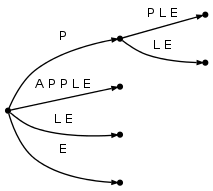
\includegraphics[width=0.5\textwidth]{suffixtree03/suffix-tree-apple}
  \caption{APPLE对应的后缀树}
  \label{suffixtree:fig:suffix-tree-apple}
\end{figure}

我们可以总结出序列$S$的后缀树有以下几个特点:
\begin{enumerate}
\item 所有的边都对应\texttt{S}的长度至少为一的非空的子序列
\item 从根到叶子节点的路径序列和序列S的后缀一一对应
\item 所有的内部节点(根节点不一定)都有至少两个子节点
\end{enumerate}

\section{Ukkonen后缀树构建算法}
\label{sec:ukkonen}
最简单的后缀树算法是先取出序列所有的后缀,然后按照前缀树的构造方法构造序列的后缀
树。这种方法虽然简单,但是复杂度较高,不适用于数据量较大的情况。为了高效地实现重
复记录检测的模块,我们的系统实现了Ukkonen在\cite{ukkonen1995line}中提出的时间复杂
度为$O(n)$的后缀树在线构建算法。以下将以字符串\texttt{BANANA}为例,简单介绍这种在
线算法的构造过程。由于这个算法比较复杂,以下的这个例子并不能涵盖算法的所有细节。

首先我们引入3个状态变量描述某一个时刻对应的后缀树的构造状态。

第一个状态变量是\texttt{\#},表示序列中即将扫描的下一个元素的位置。初始值为0,表
示第一个元素,在以后的每轮迭代中,\#的值将加1,当\#的值和序列的长度相同时迭代终
止。
  
第二个是\texttt{activePoint},用于表示下一次要在后缀树插入新的点时的位置,为了确
定这样一个唯一的位置,我们需要一个三元组\texttt{(activeNode, activeEdge,
  activeLength)}表示\texttt{activePoint},这三个变量分别表示当前后缀树的某个节点,
该节点的某条边以及这条边上第几个元素。初始值为\texttt{(root, '', 0)},表示初始的
插入操作都在根节点\texttt{root}上进行。下面
以\reffig{suffixtree:fig:suffix-tree-apple}中的后缀树为例简要说明:若
用\texttt{root}表示根节点,则当\texttt{activePoint}为\texttt{(root, A, 3)}时意味
着下一次插入新的点的位置应该是从根节点\texttt{root}的以字母\texttt{A}开头的边的
第3个字符后面,即\texttt{root}的\texttt{APPLE}对应的边的第二个\texttt{P}字母后面
的位置。
  
第三个状态变量是\texttt{remainder},表示当前还需要往后缀树中插入几次后缀。初始值
为1。

对于我们的输入\texttt{BANANA}来说,最后一个字母是\texttt{A},这个字母在字符串之前
的某个位置中出现过(\texttt{BANANA}共有3个字母\texttt{A}),因此需要在输入串的末
尾增加一个终结符,以保证输入的最后一个字符没有在之前出现过,我们这里采用\$。因此,
原始的输入\texttt{BANANA}就变成了\texttt{BANANA\$}

一开始的时候,我们只有一个根节点,\#为0,插入后缀\texttt{B},变
成\reffig{suffixtree:fig:1}所示的图;下一轮迭代\#值增加到1,新的后缀\texttt{A}在
原来的边中没有出现,插入一条新的边,得到\reffig{suffixtree:fig:2};接下来\#增加
到2,和前一步一样,新的后缀\texttt{N}没有在原来的边中出现过,插入一条新的边,得
到\reffig{suffixtree:fig:3}。目前为止,\texttt{activePoint}和\texttt{remainder}都
没发生变化。

接下来\#加1,将导致需要插入一条新的后缀\texttt{A},但是我们发现\texttt{A}已经在之
前的边中出现过,因此这时我们不插入新的边,而将\texttt{activePoint}更新
为\texttt{(root,A,1)},\texttt{remainder}加1,此时后缀树
如\reffig{suffixtree:fig:4}所示,边数没有发生变化,但是状态变量发生了改变。下一
步\#再加1,由于此时\texttt{remainder}为2,因此我们需要将新的后缀\texttt{N}往后缀
树中插入两次。从\texttt{activePoint}出发,我们发现下一个字母正好是\texttt{N},因
此我们不再试图往后缀树中插入\texttt{N}了,而是
将\texttt{activePoint}和\texttt{remainder}分别更新为\texttt{(root,A,2)}和3。下一
轮迭代也是类似,在插入最后一个\$之前,后缀树如\reffig{suffixtree:fig:6}所示,
\texttt{activePoint}和\texttt{remainder}的值分别为\texttt{(root, A, 3)}和4。

最后一轮迭代,我们需要插入终止符\$。从此时的\texttt{activePoint}出发,发现下一个
字母和和\$并不匹配,此时我们需要往后缀树中插入\$字符,方法是
在\texttt{activePoint}对应的位置生成一个新的内部节点,并在新生成的节点的地方插入
一条边,表示\$,如\reffig{suffixtree:fig:7}所示。我们需要更
新\texttt{activePoint}的值:将\texttt{activeNode}移到根节点处(在这个例子中实际上
没有移动),对应的边是以原来的\texttt{activeEdge}的第2个字母开头的边,
即\texttt{N},\texttt{activeLength}减1。\texttt{remainder}的值也减1,变为3,也就
是我们还需要插入3次\$。接下来的两次插入和我们第一次插入时的情况一样,会新生成两个
内部节点;最后一次插入则和一开始的情况一样,我们直接在根节点处插入\$。最后完整的
后缀树如\reffig{suffixtree:fig:final}所示。

在最后的\reffig{suffixtree:fig:final}中,我们看到还有一些连接几个内部节点之间的有
向的虚线,我们之前没有提到,这是后缀链(Suffix Link)。我们例子中的后缀链都是在最
后一轮迭代插入\$时生成的。关于后缀链生成的简单的规则是:在同一轮迭代中,如果在某
一步中某个节点处发生了一次插入,则要从这一轮迭代之前生成内部节点(如果有的话)引
一条后缀链指向该节点。后缀链的作用是如果在某个带有后缀链的节点发生了插入,则在更
新\texttt{activePoint}时其中的\texttt{activeNode}将更新为沿着后缀链连接的那个节点,
而不是根节点。后缀链不影响其他的规则。限于篇幅,我们不再具体举例说明后缀链的使用
方法了。
\begin{figure}
  \centering
  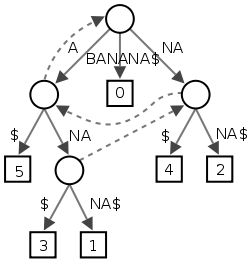
\includegraphics[width=0.5\textwidth]{suffixtree03/suffix-tree-banana}
  \caption{BANANA对应的后缀树}
  \label{suffixtree:fig:suffix-tree-banana}
\end{figure}

\section{重复记录检测算法}
\label{sec:multipldetect}

\section{本章小结}
\label{sec:summarysuffixtree}


%%% Local Variables: 
%%% mode: latex
%%% TeX-master: "../main"
%%% End: 
